\chapter{Perception}

\section{Perception of lightness \cite{wikipedia_lightness} is not linear}
\begin{figure}[H]
  %\vspace{-2ex}
  \centering
  \href{https://github.com/vicente-gonzalez-ruiz/medical_imaging/blob/main/notebooks/horizontal_vertical.ipynb}{
\includegraphics[width=\textwidth]{horizontal}}
  \caption[Perception of lightness (brightness) is not linear (1).]{In each row, the \popup{gradient}{The amount of change.} is 1 from left to right (0 in each column).}
  \label{fig:HVS_no_linear}
\end{figure}

\begin{figure}[H]
  %\vspace{-2ex}
  \centering
  \href{https://github.com/vicente-gonzalez-ruiz/medical_imaging/blob/main/notebooks/horizontal_vertical.ipynb}{
\includegraphics[width=\textwidth]{horizontal_vertical}}
  \caption[Perception of lightness is not linear (2).]{In each row and column, the \popup{gradient}{The amount of change.} 1 from top to bottom and left to right .}
  \label{fig:HVS_no_linear}
\end{figure}

\section{Perception of the lightness decreases with the spatial frequency}
\begin{figure}[H]
  %\vspace{-2ex}
  \centering
  \href{https://github.com/vicente-gonzalez-ruiz/medical_imaging/blob/main/notebooks/CSF.ipynb}{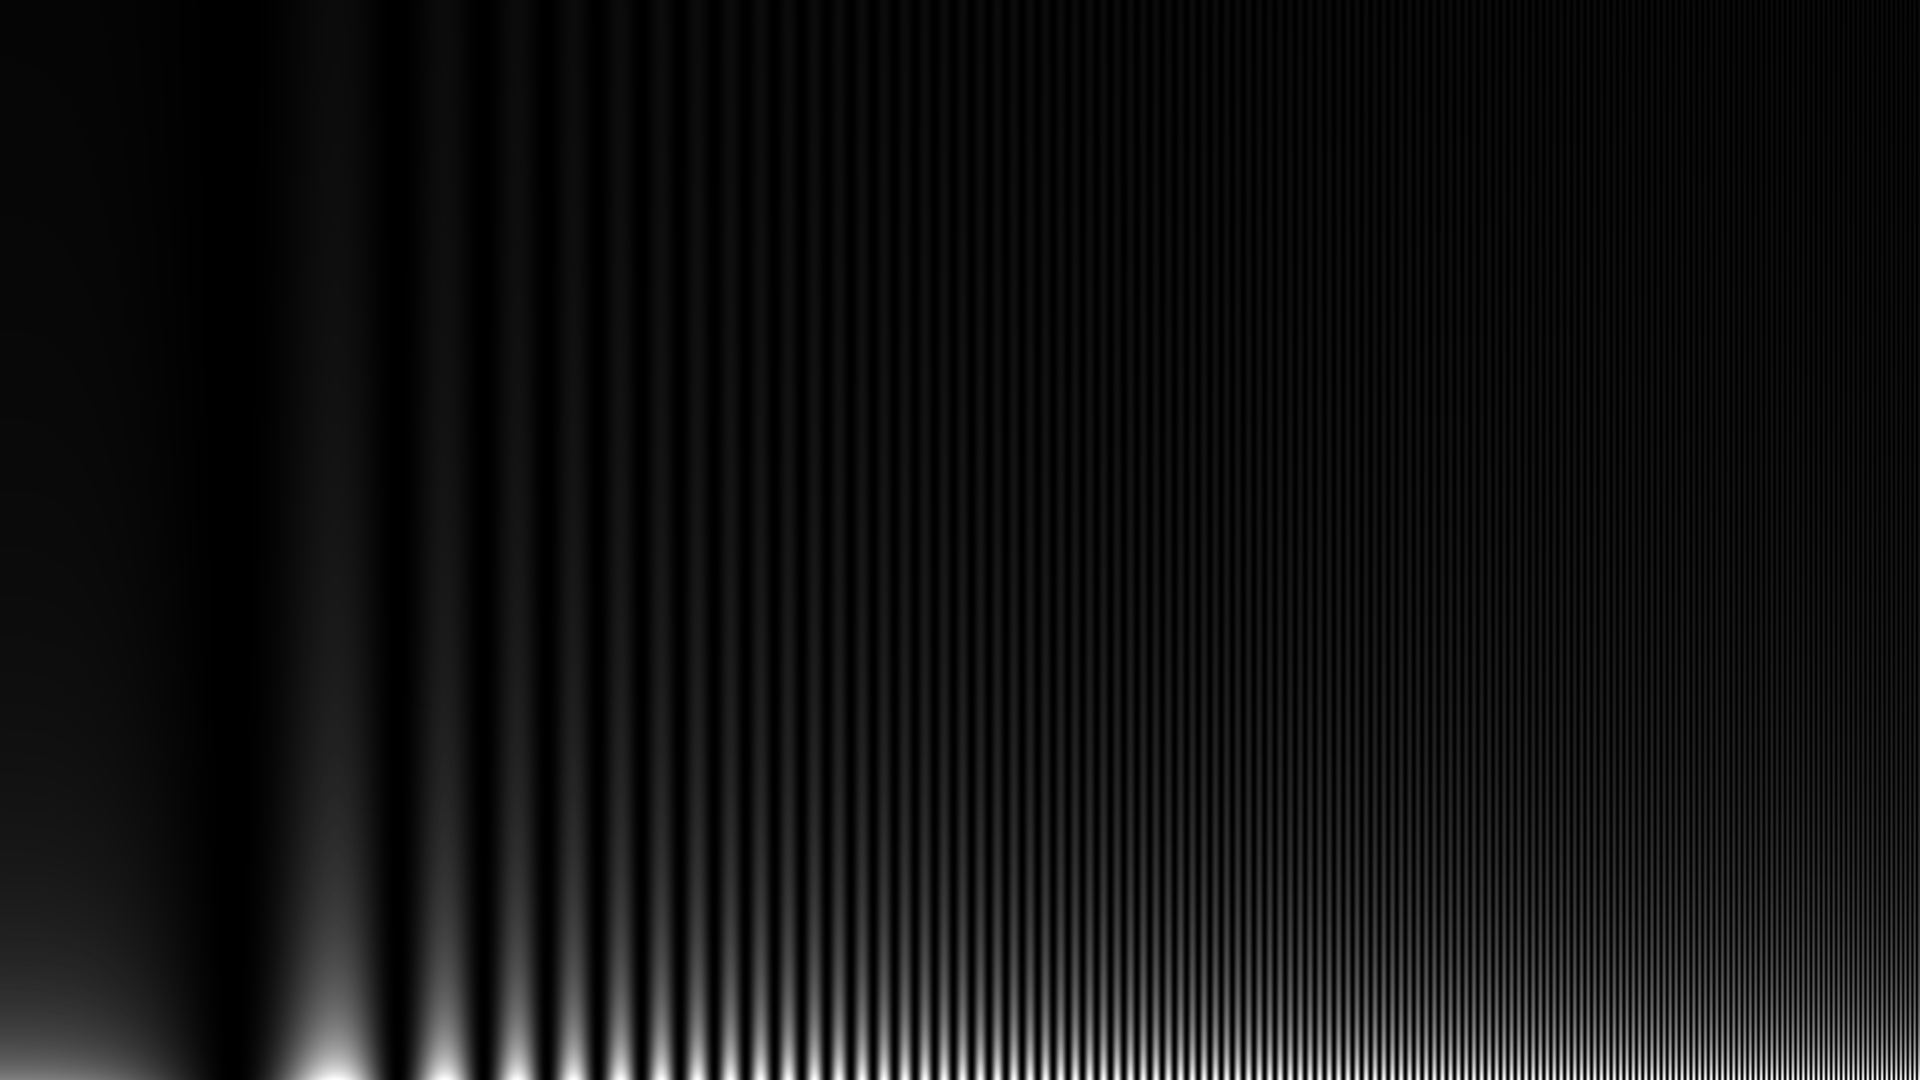
\includegraphics[width=0.60\textwidth]{CSF}}
  \caption[Lightness VS spatial frequency (the \gls{CSF}).]{The
    \gls{CSF}. Going from top to bottom, the gradient is 1 vertical
    for all the columns. Horizontally, the spatial frequency increases
    from left to right.}
  \label{fig:CSF}
\end{figure}

\section{Perception of lightness depends on the luminance of the context}
\begin{figure}[H]
  %\vspace{-2ex}
  \centering
  \href{https://github.com/vicente-gonzalez-ruiz/medical_imaging/blob/main/notebooks/stairs.ipynb}{
\includegraphics[width=0.9\textwidth]{stairs}}
  \caption[Lightness VS surrounding luminance (1).]{All the pixels of a block have the same value.}
  \label{fig:stairs}
\end{figure}

\begin{figure}[H]
  %\vspace{-2ex}
  \centering
  \href{https://github.com/vicente-gonzalez-ruiz/medical_imaging/blob/main/notebooks/same_squares.ipynb}{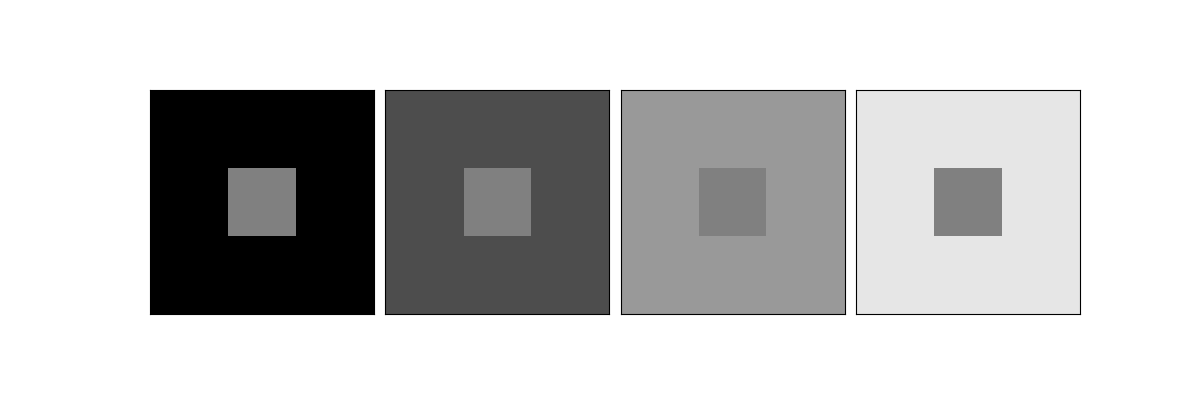
\includegraphics[width=0.8\textwidth]{same_squares}}
  \caption[Lightness VS surrounding luminance (2).]{All the internal squares have \popup{the same luminance}{All the pixels of all the squares have the same pixel value}.}
  \label{fig:squares}
\end{figure}

\section{Perception of the luma VS the visualization time}
\begin{itemize}
\item The perception of the intensity depends on the visualization time.
\begin{figure}[H]
  \vspace{-0ex}
  \centering
  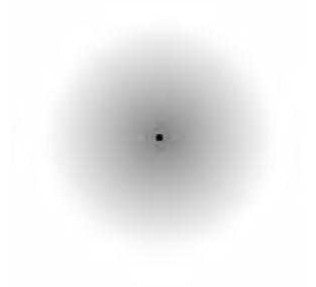
\includegraphics[width=0.35\textwidth]{punto_y_difuminado}
  \caption[Effect of visualization time in the perception of the luminance.]{Effect of the visualization time in the perception of the luminance (look to the central point for a while).}
  \label{fig:luminance_vs_visualization_time}
\end{figure}
\end{itemize}

\section{Noise masking}
\begin{itemize}
\item The perception of the structures depends on the type and intensity of the noise.
\begin{figure}[H]
  %\vspace{-2ex}
  \centering
  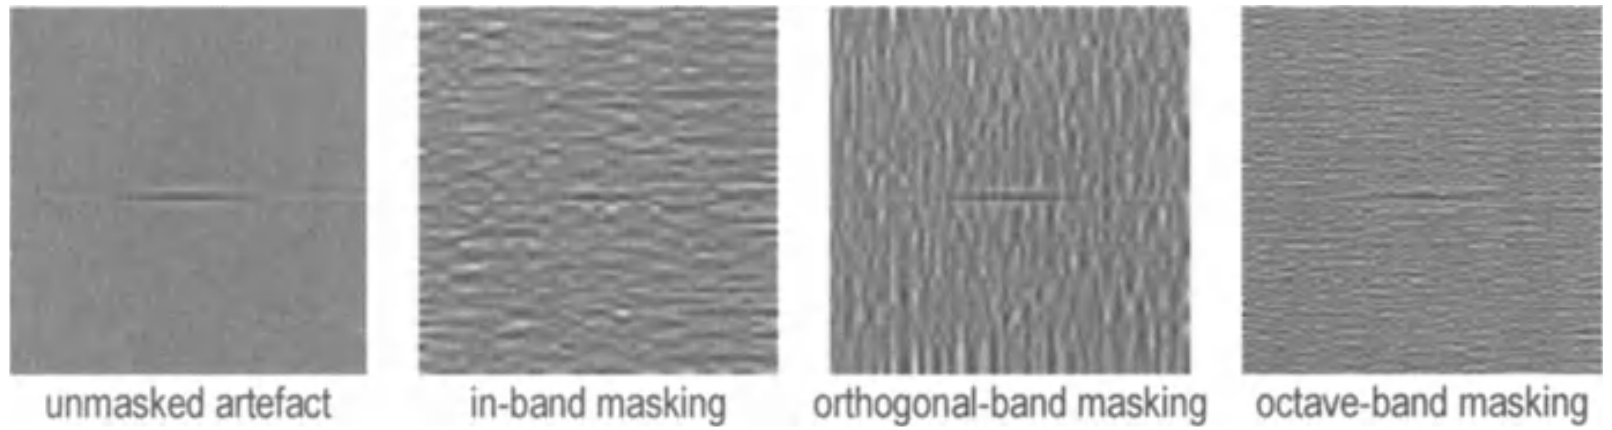
\includegraphics[width=1.0\textwidth]{noise_masking}
  \caption[Noise masking effect.]{Effect of the noise texture in the perception of the luminance (different effects of Gaussian noise in the wavelet domain).}
  \label{fig:noise_masking}
\end{figure}
\end{itemize}
